\chapter{Yhteenveto}%
\label{ch:yhteenveto}

\section{Tulokset}

Koulutettu malli vaikuttaa melko käyttökelpoiselta. Tärkeimpänä tuotoksena kuitenkin on datasetin prosessointiin toteutetut työkalut.
Vaikka täydellistä tapaa ei löydettykään, on lopputuloksesta silti nähtävissä, että yritetty datankäsittely on mahdollista.
Käytetyt tavat segmentoitujen alueiden poistamiseen näyttivät toimivan melko hyvin.
Erityisesti vertikaalinen pyyhkäisy alueen ollessa kuvan keskellä tuotti hyviä tuloksia.
Myöskin koulutusdatan ominaisuuksiin perustuva "polttopisteeseen" perustuva pyyhkäisy tekniikka vaikutti lupaavalta.
Ongelmia kuitenkin tuotti datan epätarkkuus.
Etenkin syvyysdata oli usein epätarkkaa segmentaatioon verratuuna. Tämä johti tilanteisiin, joissa pyyhkäisyn alku lähti virheellisestä syvyydestä ja koko lopullinen data oli pilalla. Yleinen ongelma oli myös pyyhkäisyn alkaminen kuvan ulkopuolelta.
Näissäkin tilanteissa pyyhkäisyn alku saattoi alkaa väärästä syvyydestä.

Mallin tuottamat tulokset olivat melko hyviä sen oman datan kanssa.
Kuitenkin ulkopuolisen datan kanssa lopullisen mallin tuotokset ovat hyvin epätarkkoja Kuva \ref{fig:ulkoinen}.
On nähtävissä että malli alkaa muodostua oikeaan suuntaan mutta se tarvitsisi paljon erilaista dataa toimiakseen.

\begin{figure}[h]
\centering
\pdftooltip{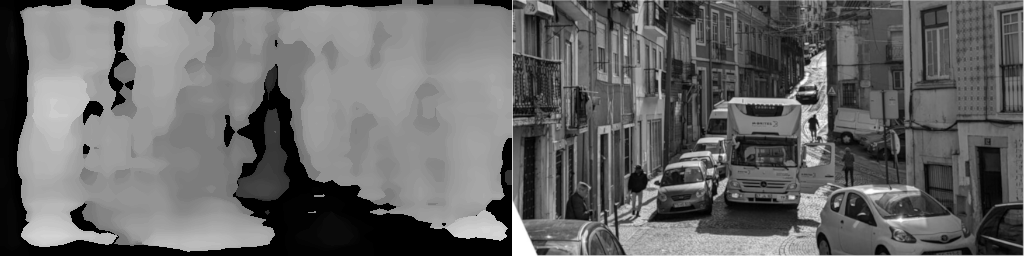
\includegraphics[width=\textwidth]{figures/outside_image.png}}{ulkoinen}
\caption{Mallin ulkopuolisista kuvista arvioitu tulos}
\label{fig:ulkoinen}
\end{figure}

Yleisesti ottaen kuitenkin työn tuottaman mallin tuloksiin voidaan mielestäni olla tyytyväisiä.
Jos tarve tämänkaltaiselle mallille kasvaa tarpeeksi suureksi, pystyy tämänkaltaisilla tekniikoilla dataa jalostamaan melko varmasti.
Ja mallin antama "sumea" tulos on riittävän tarkka sen hyödyntämiseen esimerkiksi likimääräisten 3d mallien sijoittamiseen kuvien päälle.

\section{Käyttökohteet}

Nykyisellään ainoa realistinen käyttökohde on itseajavien autojen ajoreittien suunnittelussa.
Kuitenkin jos saataisiin segmentointi ja syvyysdataa esimerkiksi ilmakuvista tai sisätiloista, voisi tätä mallia käyttää myös niiden skannaamiseen.

Mallin käyttäminen näihin tarkoituksiin ei pitäisi olla mikään ongelma, todennäköisesti ongelma olisi sama kuin nykyiselläänkin, eli datan muokkaus.
Kuitenkin käytetyt tekniikat ja luodut skriptit pitäsi olla täysin käytettävissä minkä tahansa stereodatan kanssa.
Segmentointidatan ei tarvitse olla samasta lähteestä, jos löydetään luotettava malli tai ollaan valmiita manuaaliseen läpikäyntiin.
Kuvattavasta kohteesta riippuen, nykypäivänä saatavilla olevat segmentaatio mallit voisi nähdä tarpeeksi luotettavaksi automaattiseen generointiin.

\section{Kehitysehdotukset}


Jos mallia optimoisi jollekkin pienemmälle verkolle sitä voisi ajaa suoraan esimerkiksi dronessa.
Tämä mahdollistaisi esimerkiksi maaston skannaamisen ja datan välittömän käyttämisen laitteiden reitityksen suunnitteluun.
Mallia voisi ehkä myös parantaa jos ajateltaisiin lähtökohtana olevan lidar-skannaus.
Näin syvyysdata voisi olla luotettavampaa, koska lähdedatalla olisi varma totuus. 

Tämä ei ole täysin suoraan semanttista segmentationia tai muuta yleistä koneoppimista.
Tästä johtuen voisi miettiä olisiko jokin muu malli kuin semanttinen segmentationiin suunniteltu parempi.
Tämä kuitenkin olisi loputon suo ja vaatisi hyvin paljon töitä.
Se kuitenkin voisi olla tarpeellista jos malli halutaan ajaa edge laitteella niin kuin dronella. 
Tämä voisi tehostaa toimintaa huomattavasti, koska ulostulon kokoa voitaisiin todennäköisesti pienentää melko paljon, kun jokaiselle syvyydelle ei tarvittaisi omaa segmentaatio luokkaa.

Ehkä hyödyllisin jatkokehitys voisi olla loppudatan lisäanalyysi.
Jos kuvien tuottamat 3d-pisteavaruudet saataisiin yhdistettyä, voitaisiin muodostaa tilojen 3d-skannauksia.
Tämä olisi asia mikä tekisi tästä mallista oikeasti hyödyllisen ja tuotteistettavan.
Nykyisellään sen käytännön hyöty ei ole kovin suuri muuhun kuin järjestelmille jotka erikseen tätä tarvitsevat.
Mutta erilaisten tilojen 3d-skannaus ilman esteitä olisi hyödyllistä monilla aloilla; maanmittauksessa, sisustuksessa, kaupunki suunnittelussa ja monessa muussa.

Suurimpia ongelmia on kuitenkin koulutusdatan löytäminen.
Yksi kehitysidea on rakentaa data kahden mallin avulla.
Silloin voitaisiin käyttää mitä tahansa stereodataa, josta segmentoitaisiin objektit pois.
Tämä kuitenkin muuttuvalla taustalla hankaloittaisi suuresti datan validointia.
Jotta luotettavaa dataa saataisiin tulisi tilasta ottaa stereokuvia ja kaikki liikkuvat kohteet poistaa.
Tämä olisi kuitenkin vielä työläämpää kuin kuvien manuaalinen tekeminen tai valvonta.
Tälläisen datan rakentaminen voisi olla ehkä helpointa asettamalla staattinen stereo kamera ympäristöön,
josta esimerkiki minuutin odotuksen jälkeen voidaan automaattisesti suodattaa kaikki kuvassa liikkuneet kohteet.
Näin voitaisiin generoida melko monipuolista dataa, eikä dataa tarvitsisi edes suoranaisesti segmentöidä,
koska kuvista muihin vertaamalla olisi liikkuvien alueiden tunnistaminen helppoa.
Tämä tapakin on kuitenkin melko aikaa vievää kun puhutaan tarpeesta kuvata tuhansia kuvia hyödyllisen datasetin kouluttamiseen.

Koulutusdatan muodostaminen voisi myös olla tehokasta videoiden perusteella.
Kun liikkuvasta ajoneuvosta kuvataan. Pitäisi paikallaan pitäisi ainakin autojen tunnistamisen olla helppoa.
Kyn tämän yhdistäisi jonkinnäköiseen 3d mallin rakentamiseen, jonka avulla arvioitaisiin ihmisten takana olevia asioita joita ei suoraan videolta saada.
Videoiden prosessointi olisi kuitenkin kuviin verrattuna hyvin erilainen prosessi.
Kuitenkin jos tälläinen prosessointi tuotettaisiin, olisi sille datan hankkiminen hyvin helppoa.
Teoriassa staattisten kohteiden tunnistaminen olisi helppoa koska ne jäisivät kuvassa kokoajan taustalle.
Syvyyden arviointi voitaisiin suorittaa likimääräisesti ilman stereo kameraa, koska samoista kohteista olisi useita kuvia.
Näiden kohteiden sijoitus kuvissa sekä auton nopeusdatan anylsointi mahdollistaisi dispariteetti analyysin.

Vaihtoehto olisi myös generoida data tietokoneella graafisesti,
mutta se toisi omat tekniset ongelmansa, ja sen hyödyntäminen oikeassa maailmassa voisi olla melko rajallista.
Tämä vaihtoehto vaatisi paljon testaamista.
Datan tuottaminen itsessään olisi melko helppoa,
ja ehkä joillain filttereillä varustettu kuva voisi olla tarpeeksi samankaltainen generoitujen kuvien kanssa.
